\documentclass[12pt]{article}
\usepackage[utf8]{inputenc}
\usepackage[russian]{babel}
\usepackage{amssymb}
\usepackage{systeme}
\usepackage{amsmath}
\usepackage{amsthm}
\usepackage{graphicx}
\usepackage{mathtools}
\usepackage{bbold}
\usepackage{enumitem}
\usepackage{collectbox}
\usepackage{multicol}
\usepackage[margin=0.5in]{geometry}

\title{Конспекты по линейной алгебре, 2 сем}
\author{Пак Александр}

%----ENVIRONMENTS--------------%
\newtheorem{theorem}{Теорема}
\newtheorem{lemma}{Лемма}
\newtheorem{defin}{Определение}
\newtheorem*{stat}{Утверждение}
\newtheorem{corollary}{Следствие}[theorem]
\renewcommand{\thecorollary}{\arabic{corollary}}

\newenvironment{mylist}{\begin{enumerate}[noitemsep, nolistsep]}{\end{enumerate}}

\theoremstyle{remark}
\newtheorem*{remark}{Замечание}

\theoremstyle{definition}
\newtheorem*{examples}{Примеры}

%-------------------------------%

%------COMMANDS-----------------%
\newcommand{\N}{\numberset{N}}
\newcommand{\Q}{\mathbb Q}
\newcommand{\R}{\mathbb R}
\newcommand{\Z}{\mathbb Z}
\newcommand{\0}{\mathbb{0}}
\newcommand{\mybox}{
	\collectbox{
		\setlength{\fboxsep}{1pt}
		\fbox{\BOXCONTENT}
	}
}
\newcommand{\E}{\mathcal{E}}
\newcommand{\A}{\mathcal{A}}
\newcommand{\B}{\mathcal{B}}
%-------------------------------%

\graphicspath{ {./imgs/} }

\begin{document}
	\pagenumbering{gobble}
	\maketitle
	\newpage
	\pagenumbering{arabic}
	\setcounter{section}{6}
	\tableofcontents
	\newpage
	
	\section{Линейные отображения}
	
	\subsection{Основные определения}
	\begin{defin}
		$U, V$ -- линейные пространства над полем $K(\R/ \mathbb{C})$\\
		Линейным отображением $\A$ называется $\A: U \rightarrow V$, обладающее свойством линейности:\\
		$\forall \lambda \in K, \forall u, v \in U\\ 
		\A(u + \lambda v) = \A(u) + \lambda \A(v)$
	\end{defin}
	
	\begin{remark}\hfill
		\begin{mylist}
			\item Записываем не $\A(u)$, а $\A u$
			\item "Поточечно" выполняются все арифметические операции, свойственные функциям
			\item $\A\0_U = \0_V$
		\end{mylist}
	\end{remark}
	\begin{examples}\hfill
		\begin{mylist}
			\item $\0$ -- нулевое отображение $U \rightarrow V$\\
			$\forall u \in U: \0u = \0_v$
			\item $\mathcal{E}$ -- тождественное отображение: $V \rightarrow V$\\
			$\forall v \in V: \mathcal{E}v = v$ 
			\item $U = V = P_n$ -- многочлены степени до $n$
			\\$\A: V \rightarrow V$\\
			$\A p = p'(t)$ -- дифференциальный оператор\\
			$\A(p_1 + \lambda p_2) = (p_1 + \lambda p_2)' = p_1' + \lambda p_2' = \A p_1 + \lambda \A p_2$\\
			Линейное отображение 
			$\A = \frac{d}{dt}$
			\item $U = \R^n \ V = \R^m\\
			\A = (a_{i j})_{m\times n}\\
			\A: x\in U \rightarrow y = \A x \in V\\
			x_1 + \lambda x_2 \in \R^n \rightarrow y = \A(x_1 + \lambda x_2) = \A x_1 + \lambda \A x_2$
			\item $U \cong V$. То есть отображение, на котором строится изоморфизм является линейным.
		\end{mylist}
	\end{examples}
	\begin{defin}$\lambda \in K \ \A: U\rightarrow V$\\
		Произведение линейного отображения на скаляр называется линейное отображение \\
		$\B = \lambda \A \\
		\B: U \rightarrow V \ \forall u \in U \ \B u = \lambda \A u$
	\end{defin}
	\begin{defin}
		Суммой линейных отображений $\A, \B: U \rightarrow V$ называется $\mathcal{C}: U \rightarrow V\\
		\forall u \in U \ \mathcal{C}u = \A u + \B u$
		\mybox{
			$\mathcal{C} = \A + \B$
		}
	\end{defin}
	
	\begin{defin}
		$-\A$ -- отображение противоположное $\A$\\
		$\forall u \in U \ (-\A)u = -1 \cdot \A u$
	\end{defin}
	
	$L(U, V) = Hom_K(U, V) = Hom(U, V) = \mathcal{L}(U, V)$\\
	$L(U, V)$ -- множество всех линейных отображений из $U$ в $V$.\\
	Линейное отображение = гомоморфизм с операциями $\lambda \A$ и $\A + \B$\\
	Выполнены свойства 1--8 линейного пространства (проверить самим). \\Значит \mybox{$L(U, V)$ -- линейное пространство}
	\begin{defin}
		$\A \in L(U, V)\\
		Ker\A = \{u \in U \ | \ \A u = \0_v\}$ -- ядро линейного отображения. 
	\end{defin}
	\begin{defin}
		$Im\A =\{v \in V = \A u \ \forall u \in U\} = \\ \{v \in V \ | \  \exists u \in U \ v = \A u\}$ --
		образ линейного отображения.
	\end{defin}
	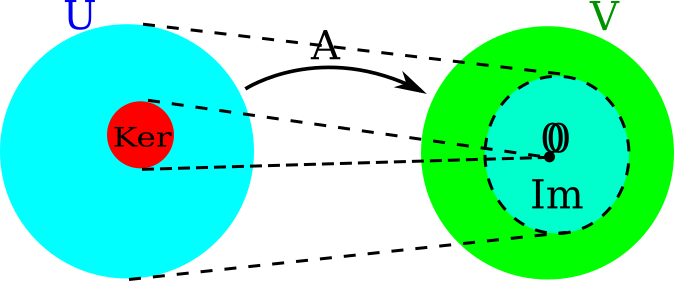
\includegraphics[width=250px]{1}
	
	Упр: $Ker\A$ и $Im\A$ - это подпространства соответственно пространств $U$ и $V$. То есть они замкнуты относительно линейных операций. \\
	Если $Ker\A$ конечномерное подпространство $U$, то \\
	\mybox{$dim \ Ker\A = def\A$} -- дефект линейного отображения.\\
	Если $Im\A$ конечномерное подпространство $V$, то \\
	\mybox{$dimIm\A = rg\A$} -- ранг линейного отображения.
	
	\begin{stat}
		$\A$ изоморфно между $U$ и $V \Leftrightarrow$ 
		\begin{mylist}
			\item $\A \in L(U, V)$
			\item $Im\A = V$
			\item $Ker\A = \{\0\}$ тривиально 
		\end{mylist}
	\end{stat}
	\begin{proof}
		$\A$ изоморфно $\Leftrightarrow$ взаимнооднозначное соответствие + линейность -- $\A\in L(U, V)$\\
		$\0_u \leftrightarrow \0_v$, т. к. изоморфизм $\Rightarrow Ker\A = \{\0\}$\\
		Пусть $Ker\A = \{\0\}$\\
		Докажем инъективность $v_1 = v_2 \Leftrightarrow u_1 = u_2\\
		v_1 = \A u_1 \ v_2 = \A u_2\\
		\0 = v_1-v_2 = \A u_1 - \A u_2 = \A(u_1 - u_2) = \0$ т. к. ядро тривиально.\\
		Сюръективность. $Im\A = V \Leftrightarrow \forall v \in V: \exists u \in U \A u = v$. Последнее и означает сюръекцию.
	\end{proof}
	\begin{defin}
		$\A \in L(U, V)$\\
		--инъективно, если $Ker\A = \{\0 \}$\\
		--сюръективно, если $Im \A = v$\\
		--биективно $\equiv$ изоморфизм, если инъекция + сюръекция.\\
		--эндоморфизм $\equiv$ линейный оператор, если $U \equiv V$\\
		$End_k(V) = End(V) = L(V, V)$\\
		--автоморфизм $\equiv$ эндоморфизм + изоморфизм. \\
		$Aut_k(V) = Aut(V)$
	\end{defin}
	\begin{defin}
		Произведением линейных отображений $\A, \B$ \\
		$\A \in L(W, V) \ \  \B \in L(U, W) \ \
		U \xrightarrow{\B} W \xrightarrow{\A} V$\\
		называется $\mathcal{C} \in L(U, V) : \mathcal{C} = \A\cdot \B$, которое является композицией функций, определяющих отображения $\A$ и $\B$.\\
		$\A\cdot \B = \A \circ \B\\
		\forall u \in U: (\A \B)u = \A(\B u)$\\
		Очевидно, $\mathcal{C}$ -- линейное отображение.
	\end{defin}
	$\Omega \xrightarrow{\mathcal{C}} U \xrightarrow{\B_{1, 2}} W \xrightarrow{\A_{1, 2}} V$\\
	Упр: \begin{mylist}
		\item $\A, \B$ изоморфизмы $\Rightarrow \A\cdot \B$ изоморфизм
		\item $(\A_1 + \A_2)\B = \A_1\B + \A_2\B\\
		\A(\B_1 + \B_2) = \A \B_1 + \A \B_2$ -- дистрибутивность
		\item $\A(\B\mathcal{C}) = (\A \B)\mathcal{C}$ -- ассоциативность
		\item $\lambda \A \B = \A \lambda \B$
	\end{mylist}
	$End(V)$ -- ассоциативная унитарная алгебра\\
	$\mathcal{E}$ -- единица $\mathcal{E}\A = \A\mathcal{E}$
	\begin{defin}
		$\A \in L(U, V)$ изоморфно.\\
		$\forall v \in V \exists! u \in U: v = \A u\\
		\A^{-1}: V \rightarrow U$\\
		\mybox{$\A^{-1}v = u$}\\
		Упр: $\A^{-1}\in L(V, U)$\\
		$\A^{-1} \A = \E_v \ \ \A\A^{-1} = \E_u$
		
	\end{defin}
	$\A\in End(U)$ -- линейный оператор
	
	$\A^{-1}\in End(V)$ -- обратный оператор
	\begin{defin}
		$U_0 \subset U \ \ \A\in L(U, V)$\\
		Сужением линейного отображения $\A$ на линейное подпространство $U_0$ называется \\
		$\A|_{U_0}: U_0 \rightarrow V \ \ \forall u \in U_0 \ \A|_{U_0} u = \A u$
	\end{defin}
	\begin{stat}
		$\A$ изоморфизм $\in L(U, V) \Rightarrow  \A|_{U_0}\in L(U_0, Im(\A|_{U_0}))$ -- изоморфизм
	\end{stat}
	\begin{examples}
		\hfil
		\begin{mylist}
			\item $\0: U\rightarrow U$ -- не сюръекция, не инъекция, эндоморфизм, не автоморфизм.
			\item $\E: U \rightarrow U$ -- автоморфизм
			\item 
			$\A = \frac{d}{dt}$ \  
			$\A: P_n \rightarrow P_n$ -- эндоморфизм, не инъекция, не сюръекция.
			\item $x\in \R^n \rightarrow y = \A x \in \R^n$ -- эндоморфизм. \\
			Сюръекция $\Leftrightarrow rg\A = n \Leftrightarrow \exists \A^{-1} \Leftrightarrow$ инъекция.\\
			То есть автоморфизм.
		\end{mylist}
	\end{examples}
	\begin{theorem}[о $rg$ и $def$ линейного отображения]
		$\A\in L(U, V)$\\
		\mybox{
			$rg\A + def\A = dimU$	
		}
	\end{theorem}
	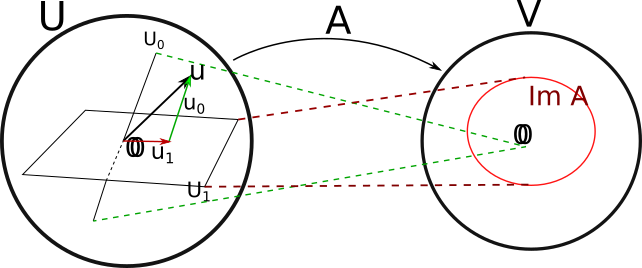
\includegraphics[width=250px]{2}
	\begin{proof}
		$U_0 = Ker\A$\\
		Дополним линейное пространство $U_1$ до пр-ва $U$:\\
		$U = U_0 \oplus U_1 \ \ \ U_1 \cap U_0 = \{ \0 \}\\
		\forall u \in U : u = u_0 + u_1$ (единственным образом)\\
		$\A u = \A u_0 + \A u_1 = \A u_1 \ \ \ \ Im\A = \A(U_1)\\
		\A_1 = \A|_{U_1}: U_1 \rightarrow Im\A$ \\
		$\A_1$ -- изоморфизм? $Im\A_1 = Im\A$ -- сюръекция\\
		$\left.\begin{array}{c}
		\forall w \in Ker\A_1 \in U_1\\
		KerA_1 \subset KerA = U_0
		\end{array}\right \}
		\Rightarrow w \in U_1 \cap U_0 = \{\0\} \Rightarrow Ker\A_1 = \{\0\}\Rightarrow \A_1$ изоморфизм.\\
		$U_1 \cong Im\A \Leftrightarrow dimU_1 = dim(Im\A)$ -- инъекция.\\
		Т. к. $U = U_0 \oplus U_1$, то $dimU = dimU_0 + dimU_1 = \underset{def\A}{dimKer\A} + \underset{rg\A}{dimIm\A}$
	\end{proof}
	\newpage 
	\begin{corollary}[Характеристика изоморфизма]
		\ \\
		$\A\in L(U, V)$ Следующие условия эквивалентны:
		\begin{mylist}
			\item $\A$ изоморфно
			\item $dimU = dimV = rg\A$
			\item $dimU = dimV\\
			Ker\A = \{\0\} \Leftrightarrow def\A = 0$
		\end{mylist}
	\end{corollary}
	\begin{corollary}
		$\A \in End(V)$ Следующие условия эквивалентны:
		\begin{mylist}
			\item $\A \in Aut(V)$
			\item $dimV =rg \A$
			\item $Ker\A = \{\0\} \Leftrightarrow def\A = 0$ 
		\end{mylist}
	\end{corollary}
	
	\subsection{Матрица линейного отображения. Изоморфизм алгебр. Преобразование матрицы линейного отображения при замене базиса.}
	\begin{multicols}{2}
		$\A \in L(U, V)\\
		\xi_1 \ldots \xi_n$ базис $U$\\
		$\eta_1 \ldots \eta_n$ базис $V$\\
		$$\forall u \in U u = \sum_{i=1}^{n} u_i\xi_i \leftrightarrow u = \left(
		\begin{array}{c}
		u_1 \\
		\vdots\\
		u_n 
		\end{array} \right)
		\in \R^n(\mathbb{C}^n)$$
	\end{multicols}
	\begin{multicols}{2}
		$$\A u = \A(\sum_{i = 1}^{n}u_i\xi_i) = \sum_{i=1}^{n}u_i\A\xi_i$$\\
		Достаточно знать, как $\A$ работает на базисных векторах $\xi_1\ldots\xi_n$
	\end{multicols}
	$Im\A = span(\A\xi_1, \A\xi_2, \ldots, \A\xi_n)$\\
	$$\A\xi_i \in V = \sum_{j=1}^{m}a_{ji}\eta_j \leftrightarrow A_i = \left(
		\begin{array}{c}
			a_{1i}\\
			a_{2i}\\
			\vdots\\
			a_{mi}
		\end{array}\right)
	\in \R^m(\mathbb{C^m})\ \ \ \ 
	a_{ji} \in \R(\mathbb{C})
	$$\\
	\mybox{
		$A = (A_1 \ldots A_i \ldots A_n) = (a_{ij})_{m\times n}$
	}
	матрица линейного отображения $\A$ относительно базисов $(\xi, \eta)$\\
	Частный случай: $\A\in End(V): \underset{e_1\ldots e_n}{V} \rightarrow \underset{e_1\ldots e_n}{V}\\
	A = (a_{ji})_{n\times n}$ -- матрица линейного оператора\\
	$$A e_i = \sum_{j=1}^{n}a_{ji}e_j$$
\end{document}